\section{Edge Computing}
\label{sec:edge-computing}

The edge represents a new tier of infrastructure envisioned to address some of
the pitfalls with the cloud for IoT applications. Cisco named it \textit{the
  fog} because the fog is a cloud close to the ground~\cite{bonomi2012fog}. CMU
chose \textit{cloudlet} to indicate this small-scale cloud
datacenter~\cite{ha2014towards, satyanarayanan2009case}. At Berkeley, we use
\textit{swarmbox} to name the hardware platform that accompanies swarm
devices. Both Smartphones and Mini PCs mentioned
in~\autoref{sec:swarm-platforms} can act as edge computing platforms. Other edge
computing infrastructure may be provided by carriers, hosted in central
offices\footnote{Often, a central office is defined as a building used to house
  the inside plant equipment of potentially several telephone exchanges, each
  serving a certain geographical area.} or cell towers~\cite{att2017edge}.

One common form of the edge computers are gateways. Many gateways provide
application-specific connectivity for IoT devices to interact with the Internet,
bridging low-power communication protocols such as BLE/802.15.4 to IP. Even when
devices can utilize more standard communication protocols such as WiFi, the
gateways still exist as downloadable applications that run on cellphones or
computers, providing custom services or user interfaces.

\begin{figure}
  \centering
  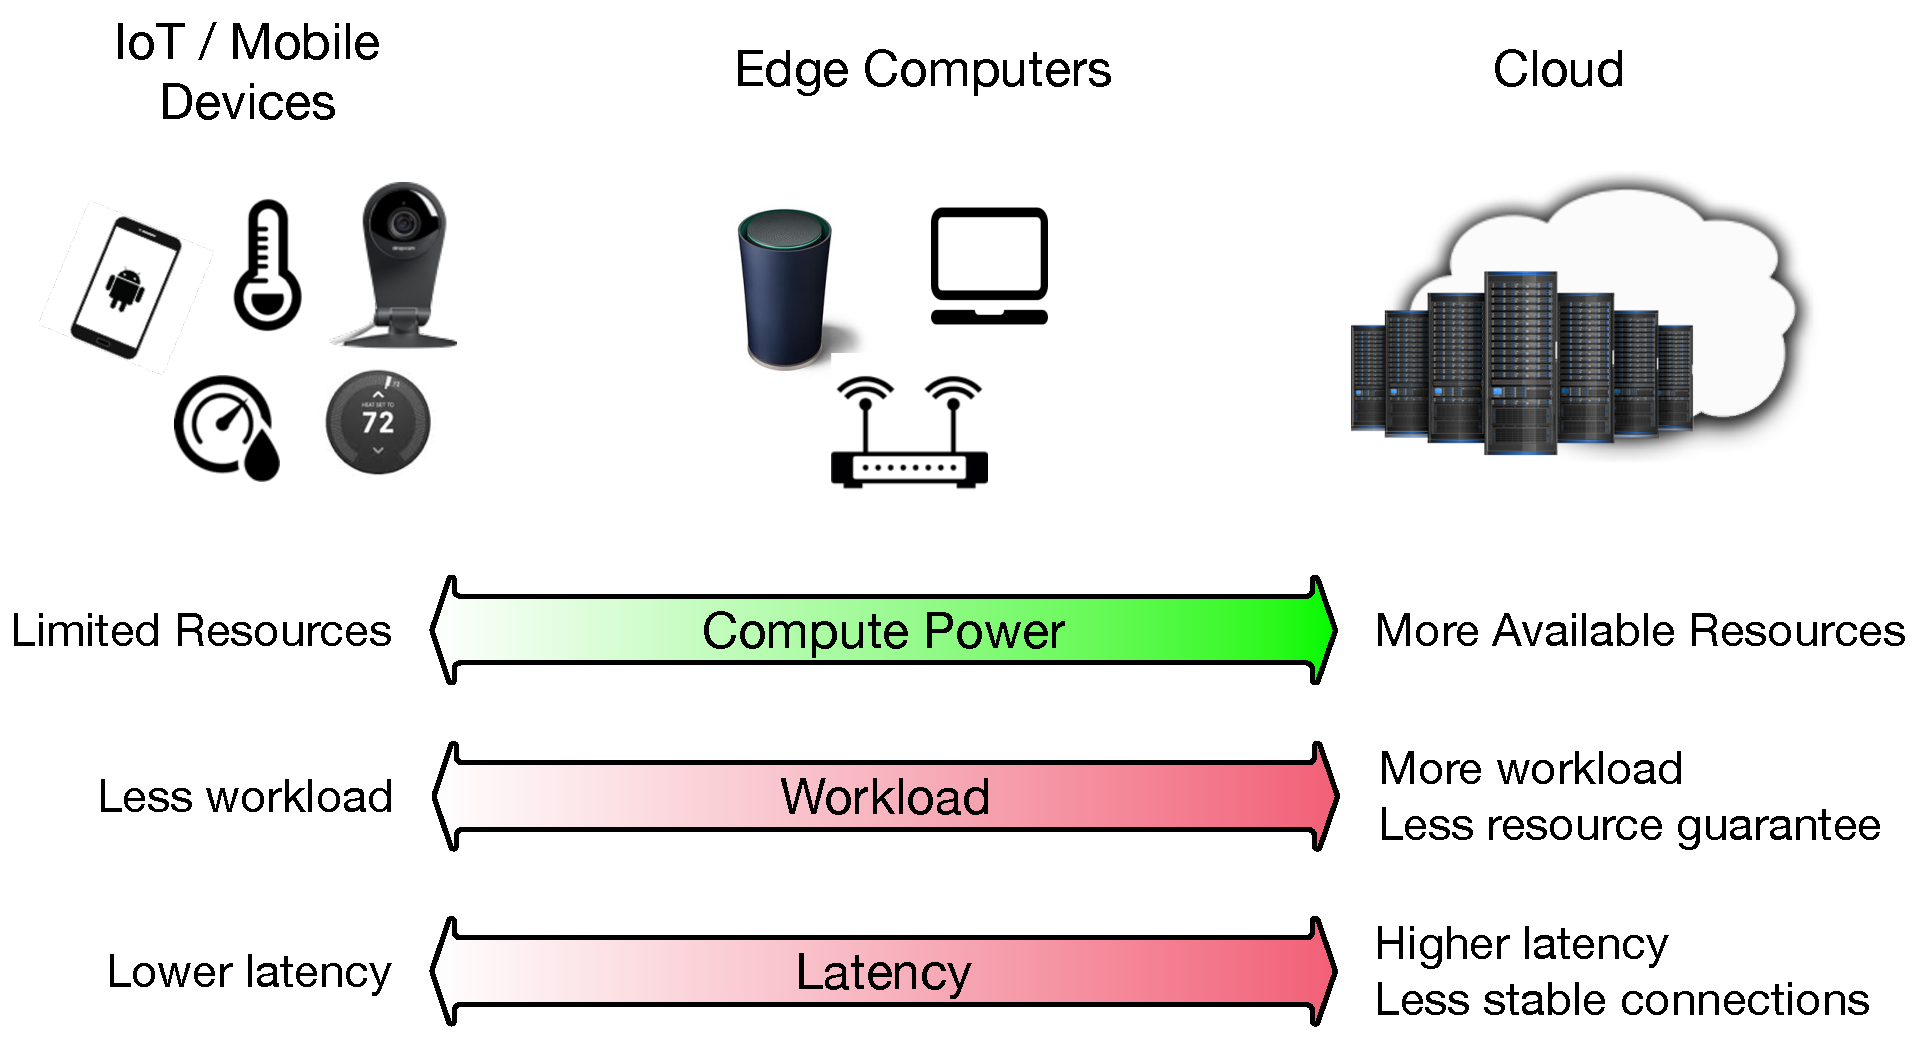
\includegraphics[width=0.85\textwidth]{figures/background.pdf}
  \caption{The characteristics of the mobile, the edge and the cloud.}
  \label{fig:edge}
\end{figure}

\autoref{fig:edge} illustrates the characteristics of the three-tier
architecture. The edge is much more powerful than end devices but less so
compared with the highly-centralized cloud. The edge serves a local area, such
as homes, buildings, or a city. As a result, it has moderate workload. The main
benefit of edge computers comes from the prime location: it sits in the middle
between IoT/mobile devices and the cloud. Applications built with the edge can
reduce network latency, keep data/information local, and tolerate cloud service
outage.

Researcher have begun to explore the benefit of edge platforms. For example, Kim
proposes an approach that leverages the edge computers as locally centralized
points for authentication and authorization to address IoT
security~\cite{kim2017securing}. Zhuo demonstrates how the edge infrastructure
can support computation offloading to achieve low
latency~\cite{chen2018application}. Mor et al.\,proposes a data-centric design
that focuses around the distribution, preservation, and protection of
information to address data privacy, scalability, durability,
etc~\cite{mor2016toward}.

While an open edge platform can realize these
benefit~\cite{zachariah1001internet}, companies tend to provide their own
gateways, such as Ninja Sphere~\cite{ninja}, SmartThings Hub~\cite{smartthings},
Wink Hub~\cite{wink}. The fact that custom gateways are an integral part of
swarm applications leads directly to ``stovepipe'' solutions or
balkanization. Data and services from one company cannot be shared or utilized
by devices from another company: connection protocols, data formats, and
security mechanisms (when present) are proprietary and often undocumented. How
to address the stovepipe issue is an active research topic. For example, Brooks
et al. proposes a component-based software architecture named ``Accessors'',
which proxies for services and things~\cite{brooks2018component}.

In addition to an open architecture, we also need to address the heterogeneous
capabilities of the edge infrastructure. As mentioned in \autoref{tab:embedded},
the swarm includes a wide spectrum of devices. It is unclear at development time
about which specific device serves as the edge. It is also difficult to make
changes to the edge, especially when it is a gateway. This is significantly from
the cloud. With its elasticity, the cloud offers the illusion of infinite
compute resources. Users can easily start another machine or even a GPU-enabled
one for heavy computation instantly. For gateways, users will need to purchase
additional devices or upgrade their existing ones: it easily takes hours or
days.

In summary, the edge offers a unique opportunity to compensate the
cloud. However, to fully realize its potentials, we need to avoid stovepipe
solutions and address challenges with the heterogeneous capabilities. This
thesis will focus on the latter.

%%% Local Variables:
%%% mode: latex
%%% TeX-master: "../background"
%%% End:
